% Ming Chen, v0.1
\documentclass{article}
\usepackage{amsmath}
\usepackage{epsfig}
\usepackage{cite}
\usepackage{graphicx}
\usepackage{spconf}


\title{reversible image watermarking based on full context prediction}
\name{Ming Chen, Zhenyong Chen, Xiao Zeng, and Zhang Xiong}
\address{School of Computer Science and Engineering\\
	Beihang University\\
	Beijing, China 100191\\
	\{mingchen@cse.\}\{chzhyong@\}\{zengxiao29@cse.\}\{xiongz@\}buaa.edu.cn}

\begin{document}
\maketitle
\begin{abstract}

This paper proposes a reversible image watermarking scheme of low distortion and relatively large
capacity, wherein prediction-errors are modified at most by 1 to embed secret bits.  Different from
most existing predictors, where only a partial prediction context is available, we provide a full
context for every pixel in our watermarking scheme. Predictors operating on full contexts are
preciser and thus produce smaller prediction-errors, which are more favorable for data embedding.
Experimental results also validate that the proposed scheme can achieve high image fidelity while
providing relatively large capacity.

\end{abstract}

\begin{keywords}
Additive prediction-error expansion, full context prediction, reversible image watermarking
\end{keywords}

\section{Introduction} \label{sec:intro}
The increasing popularity of digital multimedia application has made digital watermarking a research
hotspot recently. Digital watermarking is a technique that embeds extra host-related information
into a digital host. It can be applied to allege ownership, protect copyright, authenticate
integrity and annotate multimedia documents. Specifically, reversible image watermarking is a kind
of watermarking most applied in authentication that reversibly embeds covert information into
digital images. Its reversibility allows the host images be recovered without any loss and plays key
roles in scenarios where exact host images are crucial.  

Several kinds of reversible image watermarking have been proposed in the past few years. Tian
proposed a scheme in \cite{Tian03de}, where he expanded interpixel differences within pixel pairs to
embed data, i.e. difference expansion (DE). Based on Tian's approach, Alattar \cite{Alattar04deip}
derived a generalized integer transform, with which more differences were available for expansion
and less cost was required to record overhead information.  As another significant improvement of
the DE method, Thodi et al \cite{Thodi07pee} expanded applied it to prediction-error by expanding
differences between predicted values and original values instead of differences between paired
pixels. Thodi et al's scheme achieved higher capacity than Tian's scheme thanks to the superiority of
prediction-error in expandability. Also depending on simple integer transform, Coltus
\cite{Coltuc2007a} provided another approach of reversible watermarking, and achieved considerable
large embedding capacity. Alternatively, Lin et al \cite{Lin08tp} additively expanded the
differences within three-pixel blocks and achieved high image fidelity without sacrificing embedding
capacity.

This paper presents a reversible image watermarking scheme with full context prediction. In the
proposed scheme, distortion is constrained by limiting pixel modification to 1 through additive
expansion, and capacity is promoted by predicting every pixel within a full context with all
neighboring pixels available. The rest of this paper is organized as follows. Additive
prediction-error expansion is first described in Sect. \ref{sec:pee}. Then the proposed full context
prediction is discussed in Sect. \ref{sec:full}. Details of the algorithm are covered in Sect.
\ref{sec:algo}. Experimental results are given and evaluated in Sect. \ref{sec:results}. Finally,
conclusions and discussions are presented in Sect. \ref{sec:conclusion}.

\section{Additive prediction-error expansion} \label{sec:pee}
Additive prediction-error expansion is different from the DE approach \cite{Tian03de} in two points:
1) it expands differences by addition instead of bitshifting, 2) the expanded differences are
prediction-errors instead of interpixel differences. Tian's difference expansion using bitshifting
is 
\begin{equation}
  d' = d \times 2 + b
\end{equation}
where $d$ is the original interpixel difference and $b$ is the embedded bit. Once expanded, the
difference can be later recovered through $d = \lfloor d'/2 \rfloor$, and $b$ can be extracted by $b
= d' \bmod 2$.

Being different, the additive expansion is formulated as
\begin{equation}\label{eqn:ape}
 e' = \left\{ \begin{array}{r@{,\quad}l}
  e + sign(e) \times b & |e| = \mathit{ME} \\
  e + sign(e) \times 1 & |e| \in [\mathit{ME}+1,\mathit{LE}) \\
\end{array} \right. 
\end{equation}
where $e$ is the prediction-error, namely the difference between the pixel value and its predicted
value
\begin{equation}
 e = x - \hat{x} 
\end{equation}
and $sign(\cdot)$ is a function defined as
\begin{equation}
  sign(e) = \left\{ \begin{array}{r@{,\quad}l} 
    1 & e \ge 0 \\ -1 & e < 0 
  \end{array} \right.
\end{equation}
In (\ref{eqn:ape}), $\mathit{ME}$ is a predetermined value that maximizes the number of
prediction-errors satisfying $|e| = \mathit{ME}$ and $\mathit{LE}$ is another predetermined value
that minimizes the number of prediction-errors satisfying $|e|=\mathit{LE}$. Usually, $\mathit{ME}$
is a very small integer, whereas $\mathit{LE}$ is a larger integer with no prediction-error
satisfying $|e|=\mathit{LE}$. Note that (\ref{eqn:ape}) does not change the sign of
prediction-error, i.e. $sign(e') \equiv sign(e)$. After expansion, the watermarked pixels become $x' =
\hat{x} + e'$. It is also illustrated in Fig. \ref{fig:hist} from a histogram perspective.

\begin{figure}[t]
  \includegraphics[width=8.0cm,keepaspectratio=true,clip]{fig1.eps}
  \caption{\label{fig:hist}Illustration of additive expansion}
\end{figure}

In the extraction process, as long as $\mathit{ME}$ and $\mathit{LE}$ are known, the embedded data
can be extracted from the expanded prediction-errors through
\begin{equation}
 b = \left\{ \begin{array}{r@{,\quad}l}
  0 & |e'| = \mathit{ME} \\
  1 & |e'| = \mathit{ME} + 1 \\
\end{array} \right. 
\end{equation}
Then the inverse function of additive expansion is applied to recover the prediction-errors.
\begin{equation}
 e = \left\{ \begin{array}{r@{,\quad}l}
   e' - sign(e') \times b & |e'| \in [\mathit{ME}, \mathit{ME}+1] \\
  e' - sign(e') \times 1 & |e'| \in (\mathit{ME}+1, \mathit{LE}] \\
\end{array} \right. 
\end{equation}
Finally, we can restore the original pixels by
$x = \hat{x} + e$.

The additive prediction-error expansion is preferred to bitshifting interpixel-difference expansion
for three reasons. 1) Distortion of additive expansion ($\Delta e=e'-e \le 1$) is smaller than that
of bitshifting expansion ($\Delta d=d'-d = d + b$, the total payload does not cover the overhead
cost when threshold of $d$ is small \cite{Chang07letter}). 2) Overhead cost of additive expansion is
less expensive than that of bitshifting expansion. Additive expansion records only
overflow-potential pixels, whereas bitshifting expansion needs a location map labeling all
differences. 3) Prediction-errors are smaller and thus more expandable than interpixel-differences.
Predictors better exploit pixel correlation by operating on neighboring contexts.

\section{Full context prediction} \label{sec:full}
In \cite{Thodi07pee}, Thodi et al used a predictor borrowed from lossless image compression which
operates on a three-pixel context. Beside the one they adopted, there are still many other
predictors in the image compression community. However, most of them are constrained to operate on a
context containing just a part of the neighboring pixels, namely causal pixels, which limits their
prediction accuracy. Because, during decoding, later compressed pixels are completely unknown when
they are needed to reconstruct the same context for earlier precessed pixels. Nonetheless, it is not
the case in image watermarking. In image watermarking, it is true as the same in image compression
that later processed pixels are not known in exact during decoding. However, we know the watermarked
values of the later processed pixels. For watermarking to achieve imperceptibility, pixels are
modified within a very small range. So, though been modified, the watermarked pixels are still close
to their original values, which means they can still be contributory to prediction. Particularly, in
additive prediction-error expansion, pixels are changed at most by 1, their contributions in
prediction are not substantially discounted. Guided by this principle, we propose a predictor
operating on a full context, in which all surrounding pixels are available for more precise
prediction.

To provide full contexts for all pixels, the host image is first partitioned into non-overlapping $2
\times 2$ pixel blocks while pixels on the four borders of the host image are kept intact. Then all
pixels of the same relative position within their blocks are resampled from the host image to form
four subimages. Denote the host image as 
\begin{equation}
 I = \{ x(i,j) | (i,j) \in [1,H] \times [1,W]\} 
\end{equation}
where $W$ and $H$ are the width and height of the host image. Then the four subimages are
\begin{equation}
  \begin{array}{l}
 U_1 = \{ x(2i,2j) | (i,j) \in [1,H'] \times [1,W'] \} \\
 U_2 = \{ x(2i,2j+1) | (i,j) \in [1,H'] \times [1,W'] \} \\
 U_3 = \{ x(2i+1,2j) | (i,j) \in [1,H'] \times [1,W'] \} \\
 U_4 = \{ x(2i+1,2j+1) | (i,j) \in [1,H'] \times [1,W'] \} 
 \end{array}
\end{equation}
where $W'= \lfloor (W-2)/2 \rfloor$ and $H' = \lfloor (H-2)/2 \rfloor$. 

Now, we consider the four subimages separately in a fixed order, e.g. first $U_1$, then $U_2$, $U_3$
and $U_4$, and we apply the additive prediction-error expansion to these four subimages
respectively. For every pixel in each of the four subimages, there exists a full context containing
all its eight adjacent pixels for prediction. In this paper, we use the following full context based
predictor.
\begin{equation}
 \hat{x}(i,j) = \frac{x_w + x_n + x_e + x_s}{4} 
\end{equation}
The watermarking procedure is illustrated in Fig.\ref{fig:pass}, where watermarked pixels are
apostrophized. Let $U_i'$ be the watermarked version of $U_i$, then the full contexts of the four
subimages $U_1$, $U_2$, $U_3$, and $U_4$ are formed by pixels in $U_2 U_3 U_4$, $U_1' U_3 U_4$,
$U_1' U_2' U_4$ and $U_1' U_2' U_3'$ respectively. That is, for $U_1$, all pixels in prediction
contexts are original; for $U_2$ and $U_3$, some pixels in prediction contexts are original while
other pixels are watermarked; and for $U_4$, all pixels in prediction contexts, except some border
pixels, are watermarked.

In the extraction process, as long as the four subimages are processed in the reversed order, we can
reconstruct the same context for every pixel of all the four subimages.

\begin{figure}[t]
    \centering
    \includegraphics[width=8.5cm,height=8cm]{full_context.eps}
    \caption{\label{fig:pass}Processing procedure}
\end{figure}

\section{Algorithm description} \label{sec:algo}
In the embedding process of the proposed scheme, the four subimages are watermarked separately in a
fixed order, whereas in the extraction process, they are restored separately in the reverse order.
As all subimages are treated in the same way, to be succinct, we only discuss the embedding and
extraction process for one subimage. 
\subsection{Embedding process} \label{sec:embed}
To avoid overflow/underflow, only pixels lie between 1 and 254 are expanded for data embedding.
However, it causes an ambiguity state when the value of a pixel is changed from 1 to 0 or from 254
to 255 (pixels valued 0 or 255 are called boundary pixels). To tell whether it is expanded, we need
to first preprocess 1-value and 254-value pixels and record all pixels that cause ambiguity (called
pseudo-boundary pixels) as overhead information. Then in the second pass, all pixels lie between 2
and 253 are processed. The embedding process is described as follows.
\begin{enumerate}
  \item Predict the value of every pixel using a full context. Work out prediction-errors and find
      out $\mathit{ME}$ and $\mathit{LE}$.
  \item Apply additive expansion to all pixels equal to 1 or 254, embed part of the watermark
      message $\mathcal{W}$, and record the indices of pixels whose values become 0 or 255 to form
      overhead bitstream $\mathcal{O}$. 
  \item Concatenate $\mathcal{O}$ and the residual watermark message $\mathcal{W}'$ to form a new
      bitstream $\mathcal{N}$. Apply additive expansion to all pixels lie between 2 and 253 and
      embed $\mathcal{N}$.
\end{enumerate}

\subsection{Extraction process} \label{sec:extract}
The extraction process is itemized as follows.
\begin{enumerate}
  \item Apply the inverse additive expansion to all non-boundary pixels. Put extracted bits into
      bitstream $\mathcal{L}1$ if the restored pixels lie between 2 and 253, or else put the bits
      into bitstream $\mathcal{L}2$. Once overhead information is available in $\mathcal{L}1$,
      decode it and remove it from $\mathcal{L}1$.
  \item Identify those pseudo-boundary pixels using decoded overhead information. Apply the inverse
      additive expansion to them and put extracted bits into bitstream $\mathcal{L}3$.
  \item Reassemble $\mathcal{L}2$ and $\mathcal{L}3$ to form bitstream $\mathcal{L}4$ by ordering
      the indices of their corresponding pixels. Concatenate $\mathcal{L}4$ and $\mathcal{L}1$ to
      obtain the watermark data.
\end{enumerate}

\section{Experimental results} \label{sec:results}
The proposed scheme was implemented and tested on various standard test images using Matlab. The
performance for eight most frequently used $512 \times 512$ grayscale standard test images are
presented in Table \ref{tbl:performance}, where we use number of bits and PSNR value for measurement
of capacity and distortion. In Table \ref{tbl:performance}, all resulting PSNR values are almost as
large as 50dB. Actually, the PSNR values are guaranteed to be larger than 48.13dB, because all
pixels are altered at most by 1 ($10\log_{10}{255^2}=48.13$). The embedding capacities of the four
subimages are tabulated separately and we can see that earlier processed subimages generally provide
higher embedding capacities than later processed ones. This agrees with the fact that the predictors
are operating on some watermarked pixels for later processed subimages. However, the capacities of
later processed subimages are just a slightly lower than their predecessors. Even the capacities of
the fourth processed subimages, of which all pixels in prediction contexts are watermarked (border
pixels are not considered), are just a little lower than that of the first processed subimages, of
which all pixels in prediction contexts are original. This fact verifies our assumption that
watermarked pixels are still of significant contribution to prediction. Moreover, the pure
capacities are a little lower than the sums of the capacities of the four subimages due to overhead
costs. Nevertheless, although the overhead information is not compressed, its average cost is just
214 bits, which is negligible to the total capacity. 
\begin{table}
  \caption[Short title]{\label{tbl:performance}Performance of the proposed scheme} 
  \setlength{\tabcolsep}{1.4mm}
  \begin{tabular}{lcccccc} \hline
    Image & \multicolumn{5}{c}{Capacity (number of bits)} & PSNR\\ 
     & $U_1$ & $U_2$ & $U_3$ & $U_4$ & Pure & value  \\ \hline\hline
    Lena 	& 18341	& 17333	& 17904	& 17097	& 70627	& 49.6 \\
    Baboon	& 6342	& 6213	& 6102	& 6025	& 24634 & 48.6 \\
    Plane 	& 19658	& 19658	& 19577	& 19453	& 78154 & 50.1 \\
    Boat	& 9740	& 9474	& 9822	& 9440	& 38316	& 48.9 \\
    Tiffany 	& 12202 & 11609 & 11734 & 11519 & 46056 & 49.1 \\
    Barbara	& 12765	& 11877 & 12622 & 11797 & 48997 & 49.1 \\
    Peppers	& 10588 & 9980 	& 10040 & 9269 	& 39733 & 48.9 \\
    Goldhill	& 11482	& 11478	& 11470	& 11248	& 45630 & 49.0 \\ 
    Average	& 12640	& 12203 & 12409 & 11981 & 49018 & 49.2 \\ \hline
  \end{tabular}
\end{table}

For better evaluation of the proposed scheme, we have also included the performance of the
state-of-the-art reversible image watermarking scheme proposed by Thodi et al. \cite{Thodi07pee}.
Being similar, his scheme was also based on expansion of prediction-error. Being different, they
used bitshifting expansion rather than additive expansion and the predictor he adopted operates on a
half context instead of a full one. In their paper \cite{Thodi07pee}, six different implementations
were presented and the experimental results for four standard test images are given for all of them.
From the six, we choose the best ones for each of the four images for comparison. The result is
shown in Fig. \ref{fig:compare}, where with full context prediction and additive expansion our
scheme provides larger capacities than Thodi et al's scheme when the PSNR values are equal.

\section{Conclusions and discussions} \label{sec:conclusion}
In this paper, a high-capacity and low-distortion reversible image watermarking scheme using
additive prediction-error expansion is proposed. The additive expansion modify every pixel at most
by 1, thus only tiny distortion is induced. And the prediction is obtained from a precise predictor
operating on a full context, hence a large amount of data can be embedded. Experimental results also
verify that its embedding capacity is high and its distortion is small. 

The full context based prediction proposed in this paper is not only preciser, but also beneficial
in computation and robustness. Since the full prediction contexts for all pixels in every subimage
are not overlapped, streamlining of computation is possible. In Matlab or other vector machine, the
computation can be greatly accelerated. Moreover, since in every single subimage earlier processed
pixels are irrelated to later processed pixels, there is no error propagation. Even if part of the
watermarked image is cropped, we can still extract a portion of the embedded data.

\begin{figure}[t]
  \includegraphics[width=8.5cm, keepaspectratio=true]{fig2.eps}
  \caption{\label{fig:compare}Comparison between Thodi et al's scheme and ours.}
\end{figure}

\bibliographystyle{IEEEbib}
\bibliography{../wmbib}

\end{document}
